
\chapter{Aufbau und Analyse der ETL Prozesse}

\section{Überblick über die verwendeten Datenquellen}

Eine der Anforderungen an die Web Applikation ist es den Nutzern
aktuelle Informationen über die Wetter- und die Wellenverhältnisse in
den nächsten Tagen zu bieten. Hierfür werden die frei erhältlichen
Ergebnisse von zwei numerischen Wettermodelle verwendet, dem
\textit{Global Forecast System} und dem \textit{Wave Watch III}
Modell.

\subsection{Wettervorhersagen}

Wettervorhersagen haben das Ziel den Zustand der Erdatmosphäre zu
einer bestimmten Zeit an einem bestimmten Ort zu prognostizieren. Sie
werden meist von staatlichen oder privaten Wetterdiensten erstellt,
die sich an den Erkenntnissen der Meteorologie bedienen. Heutige
Wettervorhersagen basieren auf den aufwendig berechneten Ergebnissen
numerischer Wettermodelle.

Die Vorhersage des Wetters ist ein Anfangswertproblem, das meist in
drei Schritten gelöst wird. Im ersten Schritt, der Analyse, wird der
Ausgangszustand der Atmosphäre bestimmt. Dieser Zustand wird durch
verschiedene physikalische Größen festgelegt, die von Wetterstationen,
Satelliten, Bojen oder Flugzeugen gemessenen werden. Typische Größen
repräsentieren dabei Luftdruck, Temperatur, Wind, Wasserdampf, Wolken
und Niederschlag.

Die Modellberechnung ist der zweite Schritt, und simuliert die
Entwicklung der Atmosphäre in die Zukunft. Die Berechnung dieser
Simulation ist sehr aufwendig, weshalb meist Supercomputer eingesetzt
werden. Ergebnis der Modellberechnung ist der Zustand der Atmosphäre
zu verschiedenen Zeitpunkten in der Zukunft, dargestellt durch
physikalischen Größen.

Im letzten Schritt, der Nachbereitung, werden die Ergebnisse der
Simulation schließlich für die verschiedensten Nutzer
aufbereitet. Dies beinhaltet die Generierung von Wetterkarten,
Warnhinweisen für Technisches Hilfswerk und Feuerwehr oder die
Visualisierung von Strömungsfilmen.

\subsection{Numerische Wettermodelle}

Numerische Wettermodelle versuchen den Zustand der Erdatmosphäre und
deren Veränderung im Laufe der Zeit als mathematisches Problem zu
beschreiben. Dabei werden die physikalischen Größen und Beziehungen,
die den Zustand und die Veränderung der Atmosphäre beschreiben, als
System partieller Differentialgleichungen modelliert. Die meisten
Modelle verwenden dabei dieselben physikalischen Gesetzmäßigkeiten,
die auf den Erhaltungssätzen von Energie, Impuls und Masse
beruhen. Meist unterscheiden sie sich aber in der konkreten
mathematischen Formulierung und der numerischen Lösung der
Gleichungssysteme, weshalb die Ergebnisse verschiedener Modelle
voneinander abweichen können.

\subsubsection{Operative Wettermodelle}

Der Deutsche Wetterdienst betreibt drei verschiedene
Wettermodelle. Die lokalen \textit{COSMO-DE} und \textit{COSMO-EU}
Modelle liefern Vorhersagen für Deutschland und Europa, das globale
Modell \textit{GME} hingegen Vorhersagen für die ganze Welt. Weitere
bekannte Modelle sind das von der US-amerikanischen \textit{National
  Oceanic and Atmospheric Administration} betriebene \textit{Global
  Forecast System (GFS)} \nomenclature{GFS}{Global Forecast System}
und das neuere \textit{Weather Research and Forecasting (WRF)}
\nomenclature{WRF}{Weather Research and Forecasting} Modell, das vom
\textit{National Weather Service (NWS)} \nomenclature{NWS}{National
  Weather Service}, vom amerikanischen Militär und einigen privaten
meteorologischen Organisationen verwendet wird.

\subsubsection{Diskretisierung von Raum und Zeit}

Um die sich verändernde Atmosphäre der Erde auf ein Modell abbilden zu
können wird eine Diskretisierung von Raum und Zeit vorgenommen. Dabei
wird die Oberfläche der Erde mit einem aus Drei- oder Vierecken
bestehenden Gitternetz überzogen, und die Atmosphäre vertikal in
mehrere Luftschichten aufgeteilt. Damit wird die unendlich Zahl der
möglichen Vorhersagepunkte in der Atmosphäre auf die endliche Zahl der
so entstandenen Kreuzungspunkte reduziert. In Abbildung
\ref{gitternetz} ist das dreieckige Gitternetz des zur Zeit vom
Deutschen Wetterdienst und des Max-Planck-Instituts für Meteorologie
neu entwickelten \textit{ICON} \nomenclature{ICON}{Icosahedral
  Non-hydrostatic General Circulation Model} Wettermodells zu sehen.

\begin{figure}[h]
  \begin{center}
    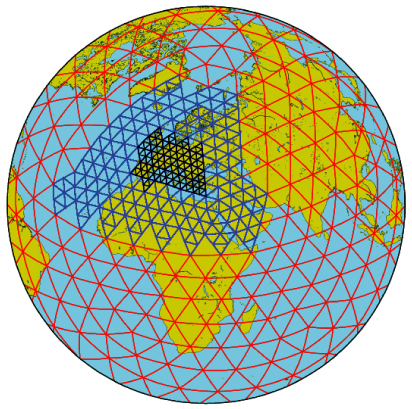
\includegraphics[height=200px]{bilder/gitternetz}
    \caption{Dreiecksgitter des ICON Wettermodells}
    \label{gitternetz}
  \end{center}
\end{figure}

Mit der Maschenweite bezeichnet man den horizontalen Abstand zwischen
zwei benachbarten Gitterpunkten. Je feiner das Gitter, bzw. je höher
die Auflösung des Modells ist, desto genauer kann die Erdoberfläche
und die darüber liegenden atmosphärischen Strukturen erfasst werden,
was sich auf die Genauigkeit der Wettervorhersage auswirkt. Die
benötigten Ressourcen zu Berechnung der Modellgleichungen steigt mit
der Anzahl der verwendeten Gitterpunkte.

Da eine sehr hohe Auflösungen selbst die Leistungsfähigkeit der
schnellsten Supercomputer übersteigt werden von den Wetterdiensten
meist verschiedene Modelle in unterschiedlichen Auflösungen
berechnet. Globale, den gesamten Globus umfassende Modelle werden mit
einer geringeren Auflösung als lokale, Länder oder Kontinente
abdeckende Modelle berechnet. Je weiter in die Zukunft prognostiziert
werden soll, desto mehr spielen aber wieder Wetterphänomene aus
Gebieten die nicht vom lokalen Modell abgedeckt werden eine Rolle. Für
Vorhersagen ab 5 Tagen in die Zukunft benötigen die lokalen Modelle
wiederum Informationen aus der gesamten Atmosphäre. Deshalb verwenden
die höher auflösenden lokalen Modelle oft Informationen als Randwerte
aus einem zuvor berechneten globalen Modell.

Die zeitliche Diskretisierung hingegen ist weniger problematisch. Die
meisten Modelle bieten mindestens Prognosen um 12 und 24 Uhr für
diejenigen Tage an, über die sich der Vorhersagezeitraum
erstreckt. Das \textit{Global Forecast System} Modell bietet
beispielsweise Vorhersagen im drei Stunden Intervall an, wobei das
lokale \textit{COSMO-DE} Modell mit einem 25 Sekunden Intervall
betrieben wird.

\subsubsection{Rechenaufwand heutiger Modelle}

In einer Präsentation
\footnote{\url{http://www.initiative-wissenschaftsjournalismus.de/fileadmin/Downloads/WissensWerte2008/B3_Majewski.pdf}}
aus dem November 2008 wurde der Rechenaufwand für die vom Deutschen
Wetterdienst betriebenen Modelle mit den dazugehörigen Kenngrößen
veröffentlicht. Damals wurden die Wettervorhersagen auf einem IBM
Power 5 System (p575) mit 52 Knoten, 416 Prozessoren und einer
Spitzenleistung von 3,1 Teraflop/s berechnet.

\begin{itemize}
\item Für Deutschland wird das \textit{COSMO-DE} Modell mit einer
  Maschenweite von 2,8 Kilometern betrieben und besteht aus ca. 10
  Millionen Gitterpunkten. Die Berechnung dauert 30 Minuten und
  liefert Vorhersagen in einem 25 Sekunden Intervall für einen
  21-stündigen Vorhersagezeitraum.
\item Das Europa umfassende Modell \textit{COSMO-EU} hat eine
  Maschenweite von 7 Kilometern, ca. 17 Millionen Gitterpunkten und
  wird mit einem Zeitintervall von 40 Sekunden erstellt. Die
  Berechnung einer 24-stündigen Vorhersage dauert 25 Minuten.
\item Das globale, die gesamte Welt umfassende \textit{GME} Modell hat
  eine Maschenweite von 40 Kilometern mit ca. 15 Millionen
  Gitterpunkten. Die Berechnung der 24 Stunden Vorhersage mit einem
  Zeitintervall von 133 Sekunden benötigt 15 Minuten.
\end{itemize}

Leider wurden während der Recherche keine genaueren Informationen
gefunden, wie sich die Berechnung der hier erwähnten Modelle auf dem
seit März 2009 beim Deutschen Wetterdienst in Betrieb genommenen
Vektorsupercomputer SX-9 der Firma NEC verhält. Die Spitzenleistung
dieses Systems beträgt momentan 4,5 Teraflop/s, die bis 2010 auf 11
Teraflop/s aufgestockt werden soll. Mit dieser neuen Anschaffung will
der Deutsche Wetterdienst unter anderem auch Wettervorhersagen mit
einer Auflösung von 2,8 Kilometern für Deutschlands Anrainerstaaten
berechnen.

\subsection{Global Forecast System}

Das \textit{Global Forecast System} ist ein globales numerisches
Wettermodell das vom \textit{National Weather Service} betrieben wird
und den gesamten Erdball abdeckt. Da die Ergebnisse der
Modellberechnung über das Internet
\footnote{\url{http://nomad5.ncep.noaa.gov/pub/gfs}} erhältlich sind
und von jedermann verwendet werden dürfen erfreut es sich einer großen
Beliebtheit. Das Modell liefert Vorhersagen bis zu 384 Stunden (16
Tage) in die Zukunft und wird mit variierenden Auflösungen viermal
täglich berechnet, jeweils um 0h, 6h, 12h und 18h koordinierter
Weltzeit (\textit{UTC}). Die ersten 180 Stunden werden mit einer
Maschenweite von ca. 40 Kilometern und einem Intervall von 3 Stunden
berechnet, die restlichen Stunden im 12 Stunden Intervall und einer
Auflösung von ca. 80 Kilometern. Vertikal wird die Atmosphäre bei
beiden Auflösungen in 64 unterschiedliche Luftschichten aufgeteilt.

Das Modell berechnet eine Vielzahl von physikalischen Größen, von
denen hier hauptsächlich die Temperatur, die Gesamtbewölkung und das
Niederschlagswasser von Bedeutung sind. Da weithin Einverständnis
darüber herrscht, dass Vorhersagen über 180 Stunden hinaus sehr
ungenau sind verwenden die hier entwickelten \textit{ETL} Prozessen
nur die ersten 180 Stunden in der hohen Auflösung.

\subsection{Wave Watch III}

Um für mehr Sicherheit auf hoher See und an Küstenregionen zu sorgen
betreibt der \textit{National Weather Service} das \textit{Wave Watch
  III} Wettermodell um Wellen vorherzusagen. Es liefert ausschließlich
Informationen über diejenigen Wellen, die durch den direkten Einfluss
von Winden entstehen. Wellen die durch andere Ereignisse wie
z.B. Gewitter, Gezeiten oder Tsunamis verursacht werden, sind in
diesem Modell nicht berücksichtigt. Da sich Wellen viel zu sehr
voneinander unterscheiden, werden nicht Vorhersagen für einzelne
Wellen getroffen, sondern über die Statistik von mehreren Wellen. Das
Modell liefert sowohl Informationen über die Wellenhöhe, Wellenperiode
und Wellenrichtung als auch über die Windstärke und die Windrichtung
an einem bestimmten Ort zu einer bestimmten Zeit.

Das Modell wird wie das \textit{Global Forecast System} viermal
täglich neu berechnet, liefert Vorhersagen im 3 Stunden Intervall für
180 Stunden in die Zukunft und die Ergebnisse sind ebenfalls frei
erhältlich
\footnote{\url{http://polar.ncep.noaa.gov/waves/index2.shtml}}. Das
globale Modell wird mit einer Maschenweite von ca. 80 Kilometern
berechnet, die lokalen Modelle mit einer Maschenweite von bis zu 20
Kilometern. Die hier entwickelten \textit{ETL} Prozesse verarbeiten
bisher nur die Daten des globalen Modells.

\section{Datenbank Design}
\subsection{Konzeptionelle Schema}
\subsection{Physisches Schema}

\section{Das GRIdded Binary Datenformat}

Die Abkürzung \textit{GRIB} \nomenclature{GRIB}{Gridded Binary} steht
für \textit{GRIdded Binary} und ist ein bitorientiertes Datenformat
zum Speichern und Übertragen von Wetterdaten. Das Format wurde von der
\textit{Kommission für Basissysteme} (\textit{CBS})
\nomenclature{CBS}{Commission for Basic Systems} der
\textit{Weltorganisation für Meteorologie} (\textit{WMO})
\nomenclature{WMO}{World Meteorological Organization} standardisiert
\footnote{\url{http://www.wmo.int/pages/prog/www/WMOCodes/Guides/GRIB/GRIB1-Contents.html}}
und wird von vielen Wetterorganisationen dazu verwendet die Ergebnisse
ihrer Modellberechnungen kompakt und plattformunabhängig zu
speichern. Insgesamt wurden drei verschiedenen Versionen spezifiziert,
von denen sich die Versionen 1 und 2 etabliert haben. Die mit der
Nummer 0 bezeichnete Version wird als veraltet angesehen und befindet
sich bei den meisten Wetterorganisationen nicht mehr im operativen
Einsatz.

\subsection{Struktur von GRIB Dateien}

Eine \textit{GRIB} Datei besteht aus eigenständigen, sich selbst
beschreibenden Datensätzen, den sogenannten \textit{GRIB}
Nachrichten. Eine Nachricht enthält dabei alle Daten eines bestimmten
Vorhersageelements, für eine auf ein Gitternetz diskretisierte
geographische Region zu einem bestimmten Zeitpunkt. Beispielsweise die
Temperaturen um 12 Uhr mittags für Europa aus dem \textit{Global
  Forecast System}, oder die signifikanten Wellenhöhen des
\textit{Wave Watch III} Modells um 9 Uhr morgens für die gesamte
Erdkugel.

Eine \textit{GRIB} Nachricht besteht wiederum aus mehreren Sektionen,
die deren Inhalt genauer beschreiben und in Tabelle \ref{tab:grib}
aufgelistet sind. Die Sektionen enthalten neben den eigentlichen Daten
u.a. Informationen über die Dimension und Auflösung des verwendeten
Gitternetzes, die Herkunft der Daten, die Art des verwendeten
Komprimierungsverfahrens und die physikalische Einheit in der die
Daten gespeichert sind.

\begin{table*}
  \centering
  {\sf
    \footnotesize
    \begin{longtable}{@{}lp{10cm}@{}}

      \toprule
      \textbf{Name der Sektion} & \textbf{Verwendungszweck} \\

      \midrule

      Indicator & Die Zeichenkette ''GRIB'', Versionsnummer, Länge der gesamten Nachricht \\

      Identification & Charakteristiken die auf alle Daten zutreffen, u.a. Herkunft der Daten, Referenzzeit und Typ des Produkts \\

      Local Use (optional) & Abschnitt für beliebige zusätzliche Informationen \\

      Grid Definition &  Definition des Gitternetzes, u.a. die Dimension, die Anzahl der Datenpunkte und die verwendete Koordinatenprojektion \\

      Product Definition &  Beschreibung der Daten. \\

      Data Representation &  Beschreibung wie die Daten repräsentiert werden. Art der Komprimierung \\

      Bitmap & Eine Bitmap, welche die Anwesenheit bzw. Abwesenheit von Datenpunkten in der nächsten Sektion signalisiert \\

      Data &  Die komprimierten Daten. Für jeden in der Bitmap existierenden Gitterpunkt ein Wert. \\

      End & Die Zeichenkette ''7777'' markiert das Ende der Nachricht \\

      \bottomrule

    \end{longtable}
  }

  \caption{Die aufeinander folgenden Sektionen einer \textit{GRIB2} Nachricht}
  \label{tab:grib}

\end{table*}

\textit{GRIB} Nachrichten können beliebig oft aneinandergereiht
werden, was eine individuelle Komposition von beliebigen Nachrichten
in einer Datei erlaubt. Dies wird in Abschnitt \ref{subsec:download}
ausgenutzt um nur ausgewählte Nachrichten aus einer größeren
\textit{GRIB} Datei zu beziehen.

\subsection{Programme zum Verarbeiten von GRIB Dateien}

Zum Verarbeiten und Lesen von \textit{GRIB} Dateien werden spezielle
Programme eingesetzt. Werkzeugen für die Kommandozeile, C-Bibliotheken
und Programmen zur Visualisierung der \textit{GRIB} Daten sind für
verschiedene Plattformen und Programmiersprachen erhältlich. Eine
Übersicht gängiger Software ist bei \textit{Wikipedia}
zusammengestellt.
\footnote{\url{http://en.wikipedia.org/wiki/GRIB\#Applications}} Zur
Weiterverarbeitung sind insbesondere die Kommandozeilenprogramme
\texttt{wgrib} und \texttt{degrib} zu empfehlen, da sie als typische
\textit{UNIX} Filter konzipiert sind und in Kombination mit
\textit{UNIX} Standardwerkzeugen wie z.B. \texttt{cat}, \texttt{curl}
oder \texttt{dd} flexibel eingesetzt werden können. Das Programm
\texttt{degrib} bietet die Möglichkeit einen Index für eine
\textit{GRIB} Datei zu generieren, mit dessen Hilfe ein wahlfreier
Zugriff nach geographischen Positionen ermöglicht wird und die
Zugriffszeiten erheblich beschleunigt.

\subsection{Inventar einer GRIB Dateien}

Die beiden Kommandozeilenprogramme \texttt{degrib} und \texttt{wgrib}
können dazu verwendet werden Inventare von \textit{GRIB} Datei zu
erstellen. Ein Inventar ist eine Art Inhaltsverzeichnis und liefert
Informationen über die in der Datei enthaltenen Nachrichten. Da
\textit{GRIB} Dateien oft mehrere Megabyte groß sind, stellen viele
Wetterorganisationen aus praktischen Gründen zusätzlich die Inventare
zur Verfügung. Ein Inventar ist zur Verarbeitung einer \textit{GRIB}
Datei zwar nicht zwingend erforderlich, vereinfacht aber den Umgang,
da nicht immer die kompletten \textit{GRIB} Dateien übertragen werden
müssen, sondern nur die sehr viel kleineren Inventare. In Abbildung
\ref{abbildung:inventar} ist der Ausschnitt eines Inventars von einer
\textit{GRIB} Datei des \textit{Global Forecast System} zu sehen. Pro
Nachricht ist in diesem Inventar eine Zeile enthalten, die unter
anderem Informationen über die Nummer der Nachricht, deren Position in
Bytes und den Zeitpunkt als auch das Element der Vorhersage, bzw. der
Analyse liefert.

\begin{figure}[h]
\begin{Verbatim}[frame=lines,framerule=0.5pt,framesep=3mm]
1:0:d=2009081812:HGT:10 mb:anl:NAve=0
2:519924:d=2009081812:TMP:10 mb:anl:NAve=0
3:812418:d=2009081812:UGRD:10 mb:anl:NAve=0
...
\end{Verbatim}
  \caption{Inventar einer \textit{GRIB} Datei des \textit{Global
      Forecast System} }
  \label{abbildung:inventar}
\end{figure}

Die zweite Zeile aus Abbildung \ref{abbildung:inventar} gibt zum
Beispiel Auskunft darüber, dass die Nachricht mit der Nummer 2 in der
\textit{GRIB} Datei an der Position 519.924 (Byte) zu finden ist, die
Werte der Nachricht für den 18. August 2009 um 12 Uhr gelten, und das
Element die Temperatur (TMP) auf einer Höhe von 10 Hektopascal (10 mb)
darstellt. Zudem handelt es sich bei den Werten nicht um eine
Vorhersage (fcst), sondern um eine Analyse (anl) für die kein
durchschnittlicher Wert (NAve=0) vorhanden ist.

\section{Extraktion aus den Quellsystemen}

\subsection{Analyse der Quellsysteme}

Sowohl das \textit{Global Forecast System} als auch das \textit{Wave
  Watch III} Modell werden viermal täglich, jeweils um 0h, 6h, 12h und
18h koordinierter Weltzeit berechnet. Danach werden die Ergebnisse in
\textit{GRIB} Dateien auf mehreren, teilweise von Unterorganisationen
der \textit{National Oceanic and Atmospheric Administration}
betriebenen Servern veröffentlicht, die verschiedensten Anforderungen
gerecht werden. Auf einigen Server sind nur die aktuellen Ergebnisse
verfügbar, andere wiederum dienen zur Archivierung und bieten eine
Historie über mehrere Jahre hinweg.

Die Ergebnisse der Modellberechnung werden in einem, meist nach Datum
und Uhrzeit strukturierten Dateisystem hinterlegt, das per
\textit{FTP} oder \textit{HTTP} exportiert wird. Die Struktur und
Benennung der Verzeichnisse und Dateien variiert dabei zwischen den
Servern, ist aber innerhalb eines Servers konsistent und folgt einem
vorhersehbaren Muster. Die \textit{URI}s der benötigten Daten können
so für einem bestimmten Server im voraus konstruiert werden und deren
Existenz mit einem der unterstützten Protokolle überprüft
werden. Dieses Verfahren kann als Anwendungsbeispiel zur
Identifizierung von Ressourcen durch vorhersehbare \textit{URI}s
angesehen werden, und ist einer der in Abschnitt
\ref{paragraph:identifizierung} beschriebenen Vorschläge der
\textit{Ressource Oriented Architecture}.

\subsubsection{Datenorganisation des Global Forecast System}

Aktuelle Daten des \textit{Global Forecast System} können in
verschiedenen Auflösung von den Servern des \textit{National Oceanic
  And Atmospheric Administration Operational Model Archive and
  Distribution System (NOMADS)} \nomenclature{NOMADS}{NOAA Operational
  Model Archive and Distribution System}
\footnote{\url{http://nomads.ncdc.noaa.gov}} bezogen werden. In
Tabelle \ref{tab:gfs_auflösungen} sind die Dateigrößen und
Bezugsquellen der \textit{GRIB} Dateien in den verschiedenen
Auflösungen dargestellt. Die Dateigröße bezieht sich dabei immer auf
eine einzelne \textit{GRIB} Datei, die alle Vorhersageelemente des
\textit{GFS} für einen bestimmten Zeitpunkt in der Zukunft enthält.

\begin{table*}[h]
  \centering
  {\sf
    \footnotesize
    \begin{longtable}{@{}ccl}

      \toprule
      \textbf{Auflösung} & \textbf{Dateigrößen} & \textbf{URI der Bezugsquelle} \\

      \midrule

      2$^{\circ}$ x 5$^{\circ}$ & 4 Mb - 4.8 Mb & \url{http://nomad5.ncep.noaa.gov/pub/gfs2p5} \\
      1$^{\circ}$ x 1$^{\circ}$ & 25 Mb - 29 Mb & \url{http://nomad5.ncep.noaa.gov/pub/gfs} \\
      0.5$^{\circ}$ x 0.5$^{\circ}$ & 200 Mb - 215 Mb & \url{http://nomad5.ncep.noaa.gov/pub/gfs_master} \\

      \bottomrule

    \end{longtable}
  }

  \caption{Dateigrößen der verschiedenen Auflösungen des GFS}
  \label{tab:gfs_auflösungen}

\end{table*}

Die in dieser Arbeit entwickelten \textit{ETL} Prozesse arbeiten alle
mit den \textit{GRIB} Dateien der höchsten Auflösung
(0.5$^{\circ}$ x 0.5$^{\circ}$). Unter der \textit{URI}
\url{http://nomad5.ncep.noaa.gov/pub/gfs_master/} sind Verzeichnisse
zu finden, die nach dem Muster \texttt{gfs\textbf{YYYYMMDD}} benannt
sind. Dabei steht \texttt{YYYY} für das Jahr, \texttt{MM} für den
Monat und \texttt{DD} für den Tag, an dem ein Modell berechnet
wurde. Beispielsweise waren die \textit{GRIB} Dateien aller
Modellberechnungen, die am 16. August 2009 durchgeführt wurden unter
der \textit{URI}
\url{http://nomad5.ncep.noaa.gov/pub/gfs_master/gfs20090816/}
aufgelistet.  \footnote{Der Server \texttt{nomad5.ncep.noaa.gov}
  verwaltet keine historischen Daten, d.h. wenn dieses Dokument
  gelesen wird sind höchstwahrscheinlich keine Daten mehr vorhanden.}

In den nach Tagen geordneten Verzeichnissen befinden sich
\textit{GRIB} Dateien die nach dem Muster
\texttt{gfs.t\textbf{XX}z.master.grbf\textbf{YY}} benannt sind. Die Zeichen
\texttt{XX} stehen dabei für den Zeitpunkt der Modellberechnung (00,
06, 12 oder 18), und die Zeichen \texttt{YY} für die Stunde der
Vorhersage in der Zukunft (00-180 im 3 Stunden Intervall). Die
Vorhersagedaten des \textit{GFS} für den 16. August 2009 um 18 Uhr
abends, die am selben Tag um 6 Uhr morgens berechnet wurden, waren
somit in der \textit{GRIB} Datei mit der \textit{URI}
\url{http://nomad5.ncep.noaa.gov/pub/gfs_master/gfs20090816/gfs.t06z.master.grbf12}
zu finden.

Eine \textit{GRIB} Datei des \textit{Global Forecast System} enthält
für einen bestimmten Zeitpunkt 63 verschiedene Vorhersageelemente und
ist zwischen 200 und 215 Megabyte groß. Die Größe aller \textit{GRIB}
Daten für einen Vorhersagezeitraum von 180 Stunden (und für den
Berechnungszeitpunkt selbst) mit einem 3-stündigen Intervall beträgt
somit $(180h / 3h + 1) * 215 Mb = 13115 Mb$. Da aber nur sehr wenige
Vorhersageelemente der \textit{GRIB} Dateien benötigt werden, wird in
Abschnitt \ref{subsec:download} ein Verfahren vorgestellt, um nur die
benötigten Elemente zu übertragen, und somit das Datenvolumen zu
reduzieren.

\subsubsection{Datenorganisation des Wave Watch III Models}

Die Daten des \textit{Wave Watch III} Modells sind ähnlich
strukturiert wie die des \textit{Global Forecast System}, und werden
in einer Auflösung von 1.25$^{\circ}$ x 1$^{\circ}$ ebenfalls auf den
\textit{NOMADS} Servern veröffentlicht. Die \textit{GRIB} Dateien
werden in Verzeichnissen hinterlegt, die nach dem Muster
\texttt{nww3\textbf{YYYYMMDD}} benannt, und unter der \textit{URI}
\url{http://nomad5.ncep.noaa.gov/pub/waves/nww3} angeordnet sind. Auch
hier ist das Datum der Modellberechnung im Verzeichnisnamen
kodiert. Das \textit{Wave Watch III} Modell hat im Vergleich zum
\textit{Global Forecast System} viel weniger Elemente, weshalb die
kompletten Daten für eine 180-stündige Vorhersage in einer einzigen
Datei gespeichert werden. Diese ist nach dem Muster
\texttt{nww3.t\textbf{XX}z.grib} benannt, wobei \texttt{XX} hier
ebenfalls für den Zeitpunkt der Modellberechnung (00, 06, 12 oder 18)
steht. Die Ergebnisse des \textit{Wave Watch III} Modells, das z.B. am
16. August 2009 um 18 Uhr berechnet wurde, konnten unter der
\textit{URI}
\url{http://nomad5.ncep.noaa.gov/pub/waves/nww3/nww320090816/nww3.t18z.grib}
bezogen werden.

Eine \textit{GRIB} Datei des \textit{Wave Watch III} Models mit 11
verschiedenen Elementen ist bei einer Auflösung von
1.25$^{\circ}$ x 1$^{\circ}$ ca. 32 Megabyte groß und enthält
Vorhersagedaten für 180 Stunden in die Zukunft.

\subsection{Partieller Download der GRIB Dateien}
\label{subsec:download}

Die eben beschriebenen Vorhersagemodelle bieten sehr viel mehr
Informationen zum Download an, als von der hier entwickelten
Anwendungen überhaupt benötigt wird. Vom \textit{Global Forecast
  System} werden im Moment lediglich 4 der 63 verschiedenen
Vorhersagelemente, und vom \textit{Wave Watch III} Modell 7 von 11
Elementen verwendet. Um nicht unnötig Bandbreite zu verschwenden, und
den Extraktionsprozess zu beschleunigen, wird hier ein Verfahren
verwendet, das in dem Dokument \textit{Fast Downloading of GRIB Files}
\footnote{\url{http://www.cpc.noaa.gov/products/wesley/fast_downloading_grib.html}}
beschrieben ist. Voraussetzung dafür ist, dass der Server das HTTP/1.1
Protokoll unterstützt, und die Inhaltsverzeichnisse der GRIB Dateien
zu Verfügung stehen.

Die aus eigenständigen und sich selbst beschreibenden Nachrichten
bestehenden GRIB Dateien werden bei der Extraktion so transformiert,
dass 

\section{Transformation der Daten}
\section{Laden der Daten}
\section{Verbesserungen}

%%% Local Variables:
%%% mode: latex
%%% TeX-master: "../community-plattform"
%%% End:
